\documentclass{ctexart}
\usepackage{geometry}
\usepackage{listings}
\usepackage{textcomp}
\usepackage{graphicx}
\usepackage[hidelinks]{hyperref}
\usepackage{hyperref}
\usepackage{appendix}
\usepackage{multirow}
\usepackage{amsmath,amssymb,amsfonts}
\usepackage[framed,numbered,autolinebreaks,useliterate]{mcode}
%记得用xelatex
% 导入首行缩进用的宏包
\usepackage{indentfirst}
\setlength{\parindent}{2em}
% 每行缩进两个汉字
\usepackage{url}
\setlength{\parindent}{0pt}
\setlength{\parskip}{18pt}
\title{\vspace{+4cm}\textbf{一年内初婚年龄分布的简单分析}}
\author{冯健齐}
\date{\today}
% //////////////////////////////////////////////////

\begin{document}

\maketitle
%目录
\newpage
\pagenumbering{Roman}
\setcounter{page}{0}
\tableofcontents
\newpage
\setcounter{page}{1}
\pagenumbering{arabic}
%标题

\section{问题背景}
\setlength{\parindent}{2em}每年结婚的人数很多,而且每个人初婚的年龄也不同,根据《婚姻法》第六条规定,结婚年龄,男不得早于二十二周岁,女不得早于二十周岁。晚婚晚育应予鼓励。由于社会节奏与时代的变化,结婚年龄应该集中分布在某个合适的数值,下面根据中国2010年人口普查网站的数据\cite{ref1}进行分析。

\section{数据的分析}
\subsection{所有年份的初婚年龄分析}
\setlength{\parindent}{2em}一共收集到1980到2010这31年的数据,为了方便观看,我们每两年分析一次,即1980,1982,1984,……,2010这16年的数据,首先绘制出这几年的数据分布。


\begin{figure}[h!]
\centering
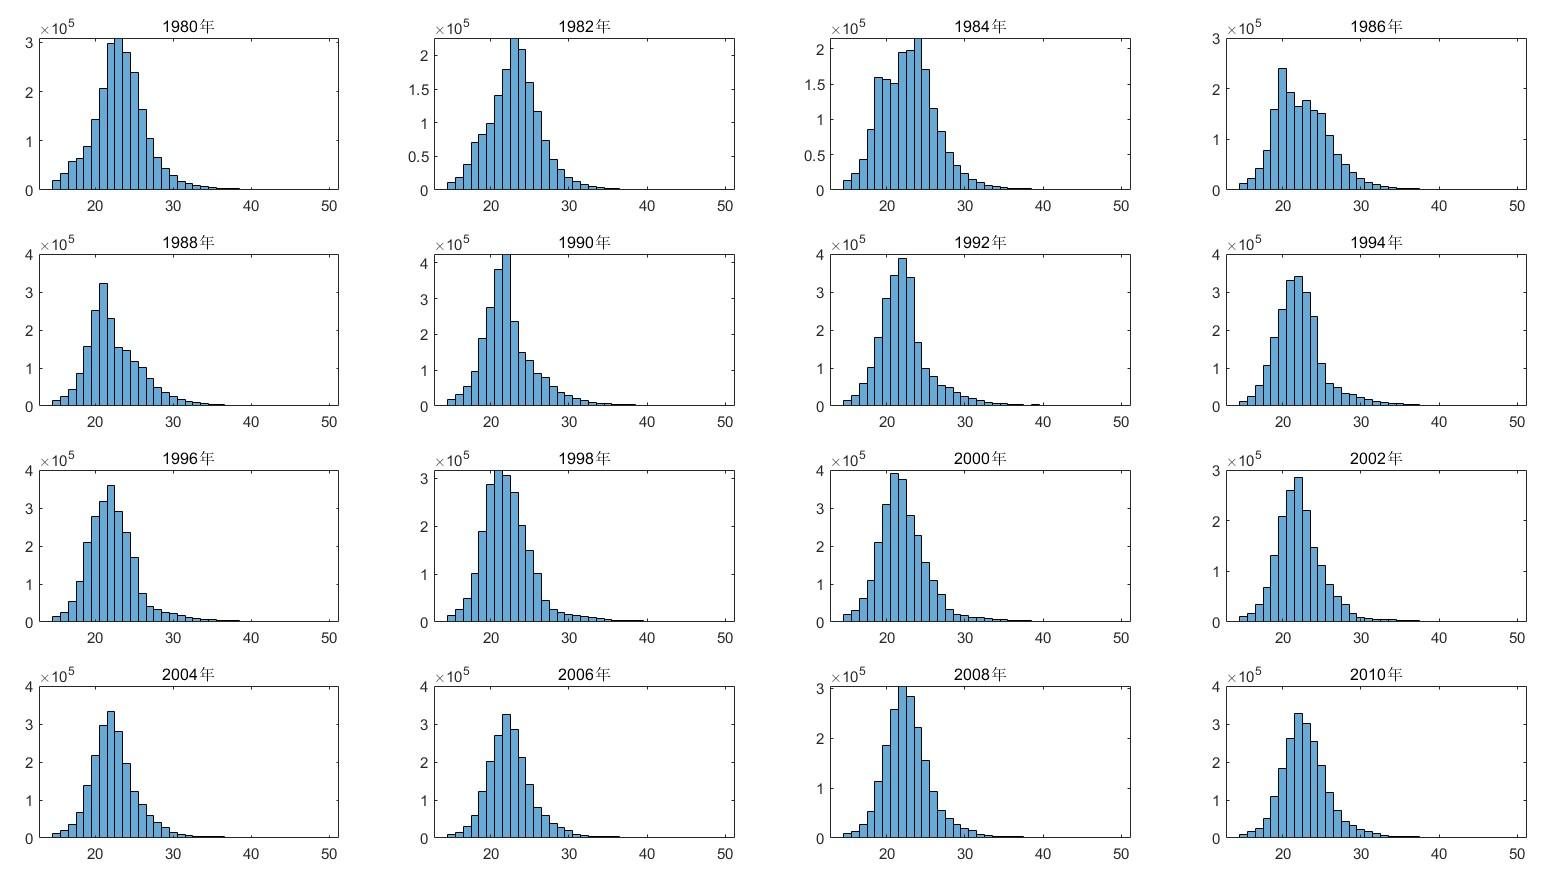
\includegraphics[width=1\textwidth]{001.JPG}
\caption{初婚年龄分布直方图}
\end{figure}


\setlength{\parindent}{2em}之后,我们绘制出所有年份下数据的分布图像。
\begin{figure}[h!]
\centering
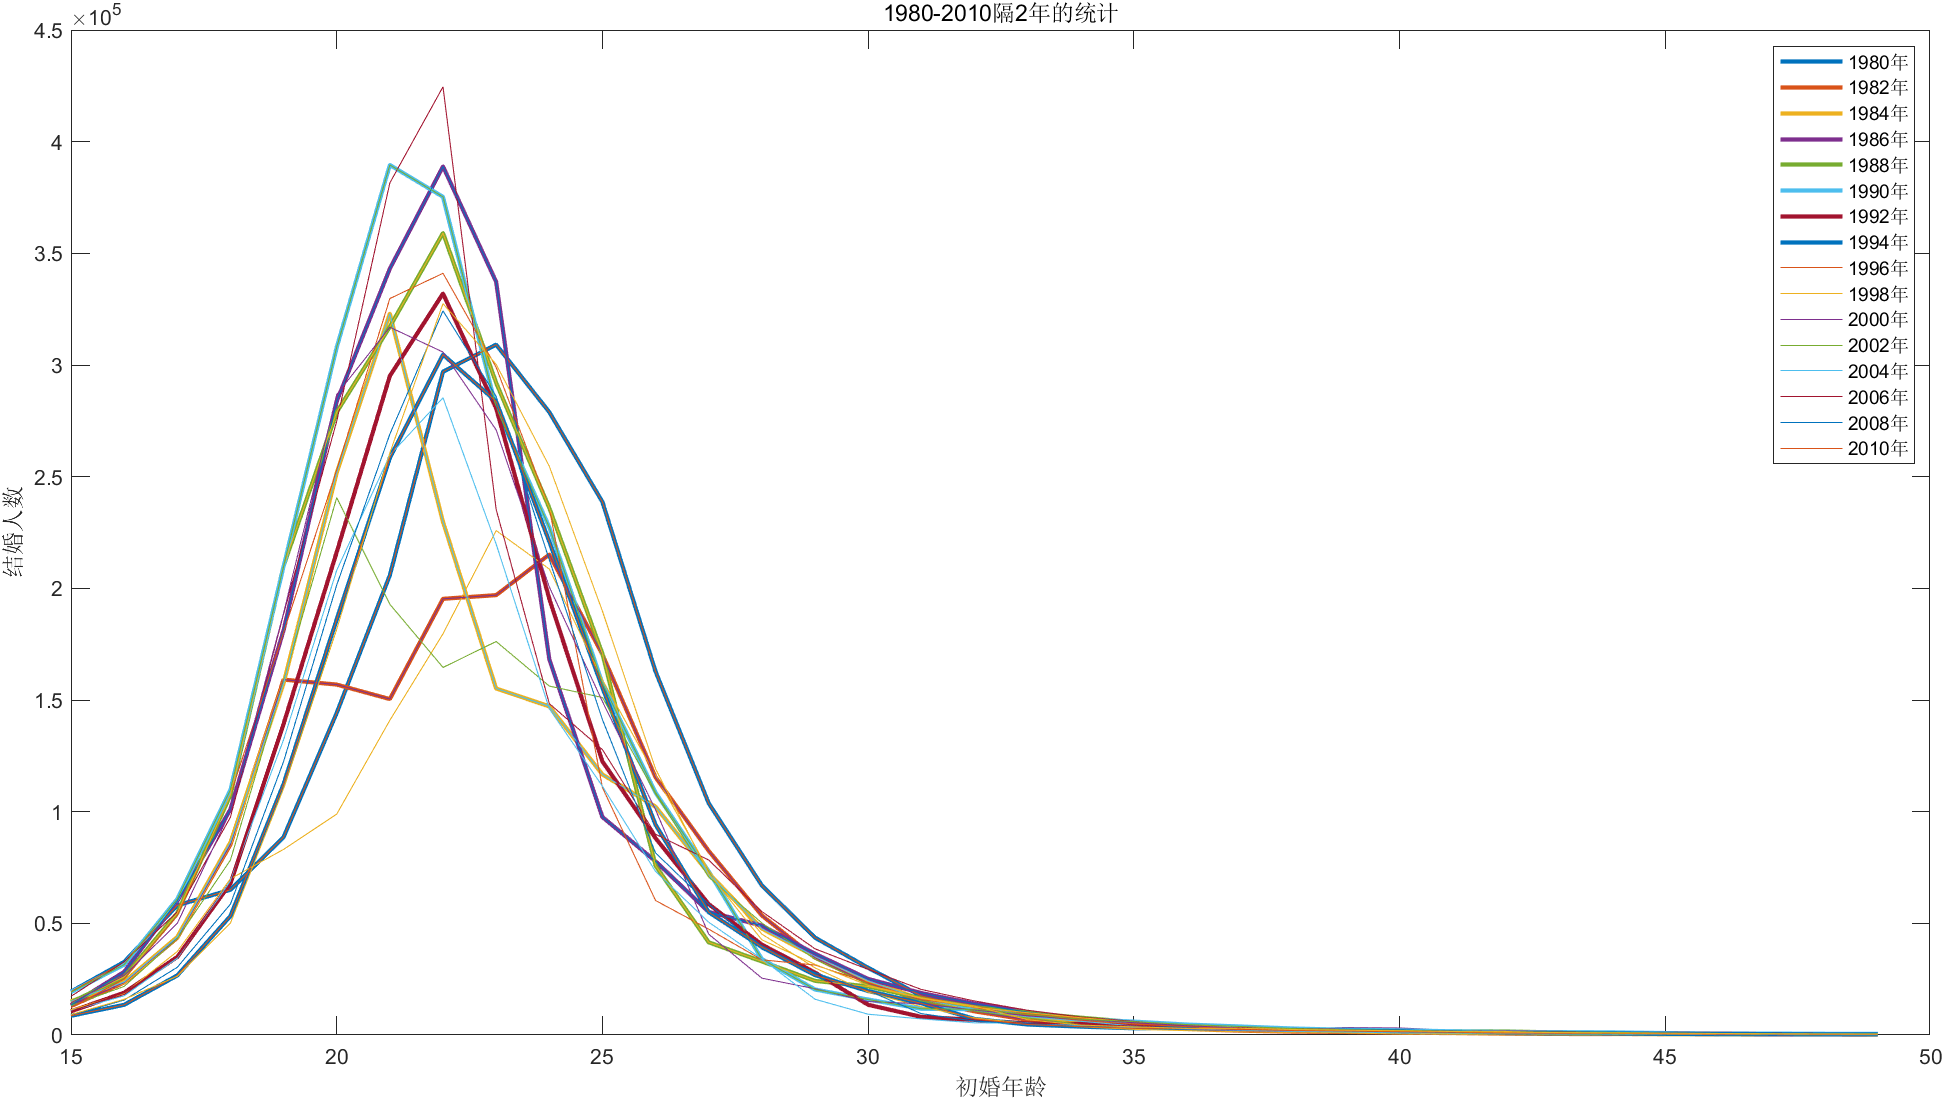
\includegraphics[width=0.9\textwidth]{002.png}
\caption{所有年份下的分布(隔2年)}
\end{figure}

\begin{figure}[h!]
\centering
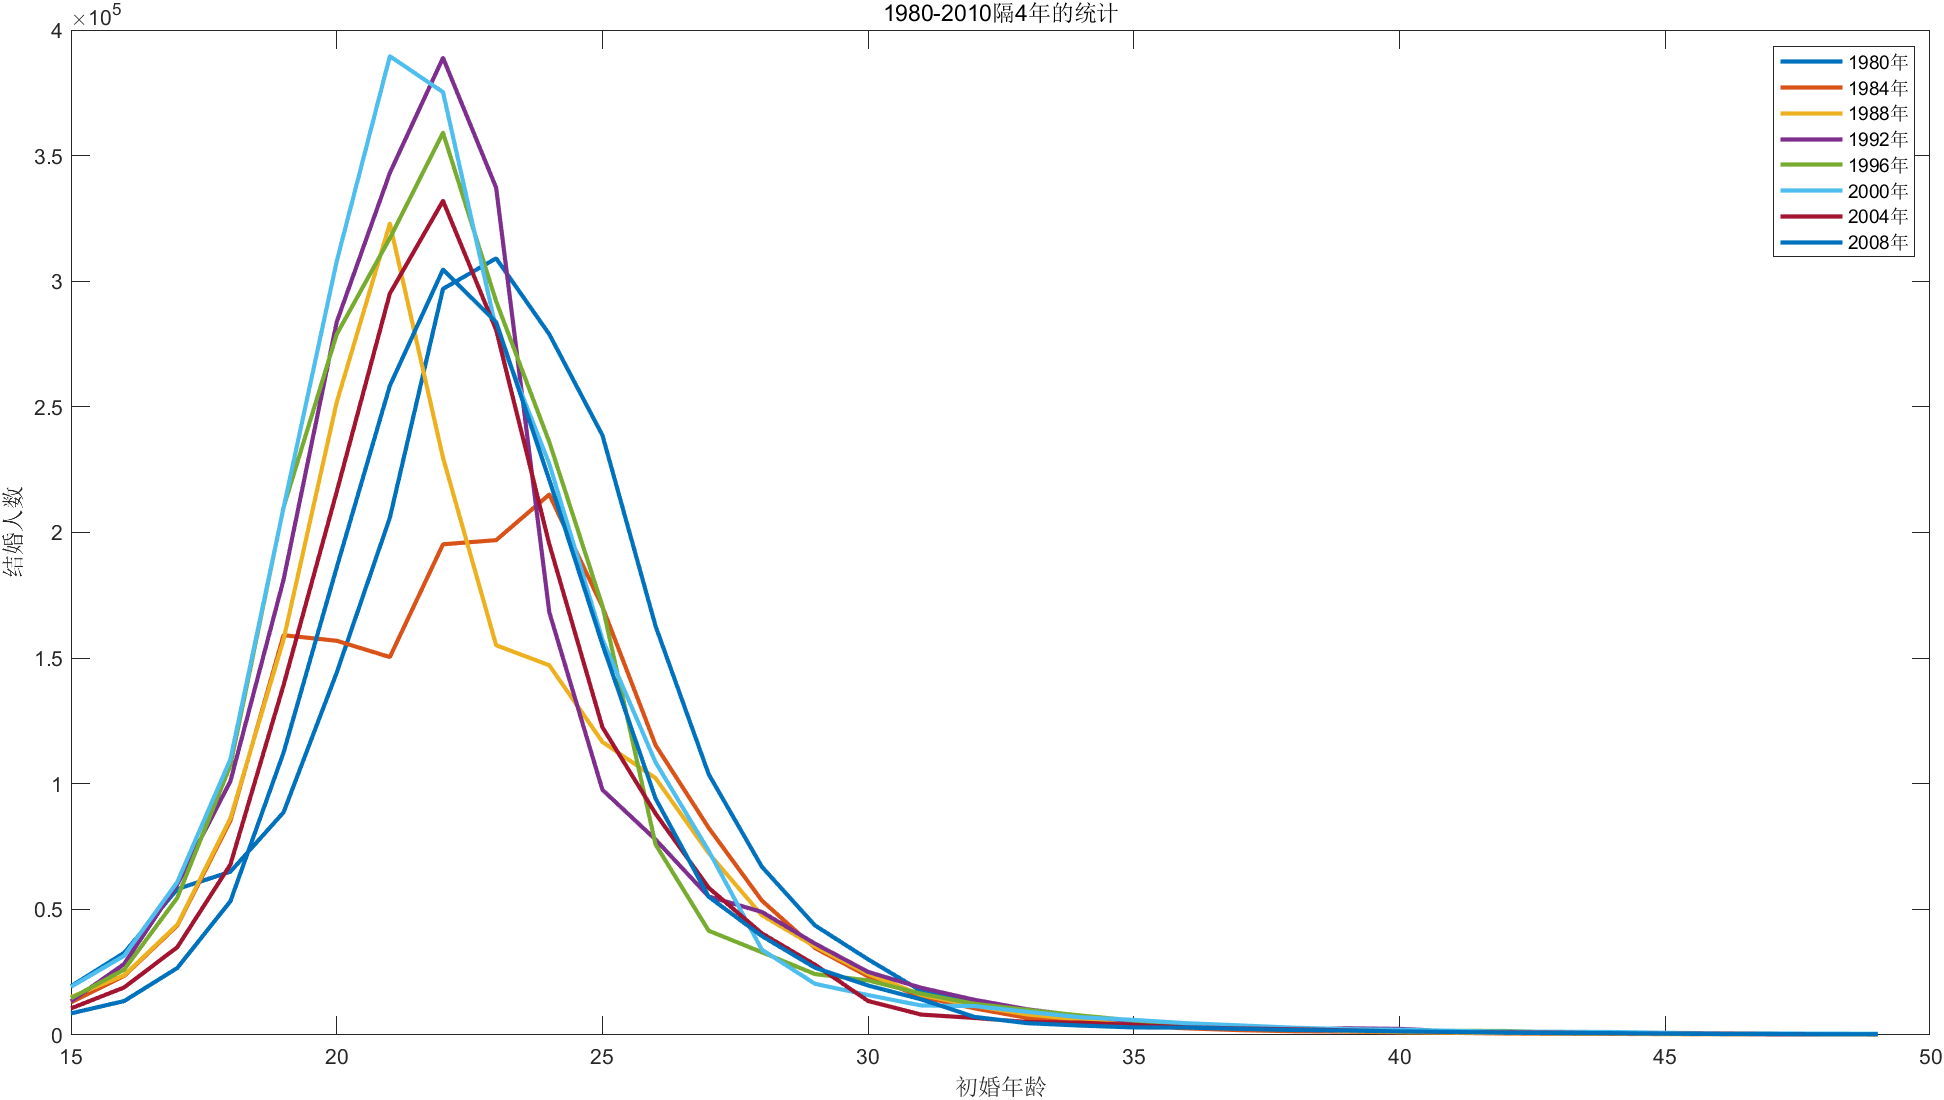
\includegraphics[width=0.9\textwidth]{003.png}
\caption{所有年份下的分布(隔4年)}
\end{figure}

从中我们也可以看出,从1980年到2010年,结婚年龄基本集中在25岁左右。下面分析其是否服从正态分布。




\subsection{每个年份的数据分析}
 \setlength{\parindent}{2em}我们对每个年份的数据进行正态分布检验,由于数据量庞大,此处用到Jarque–Bera检验。结果全为1,即不服从正态分布。随后,我们绘制出各个年份的QQ图。
 \begin{figure}[h!]
\centering
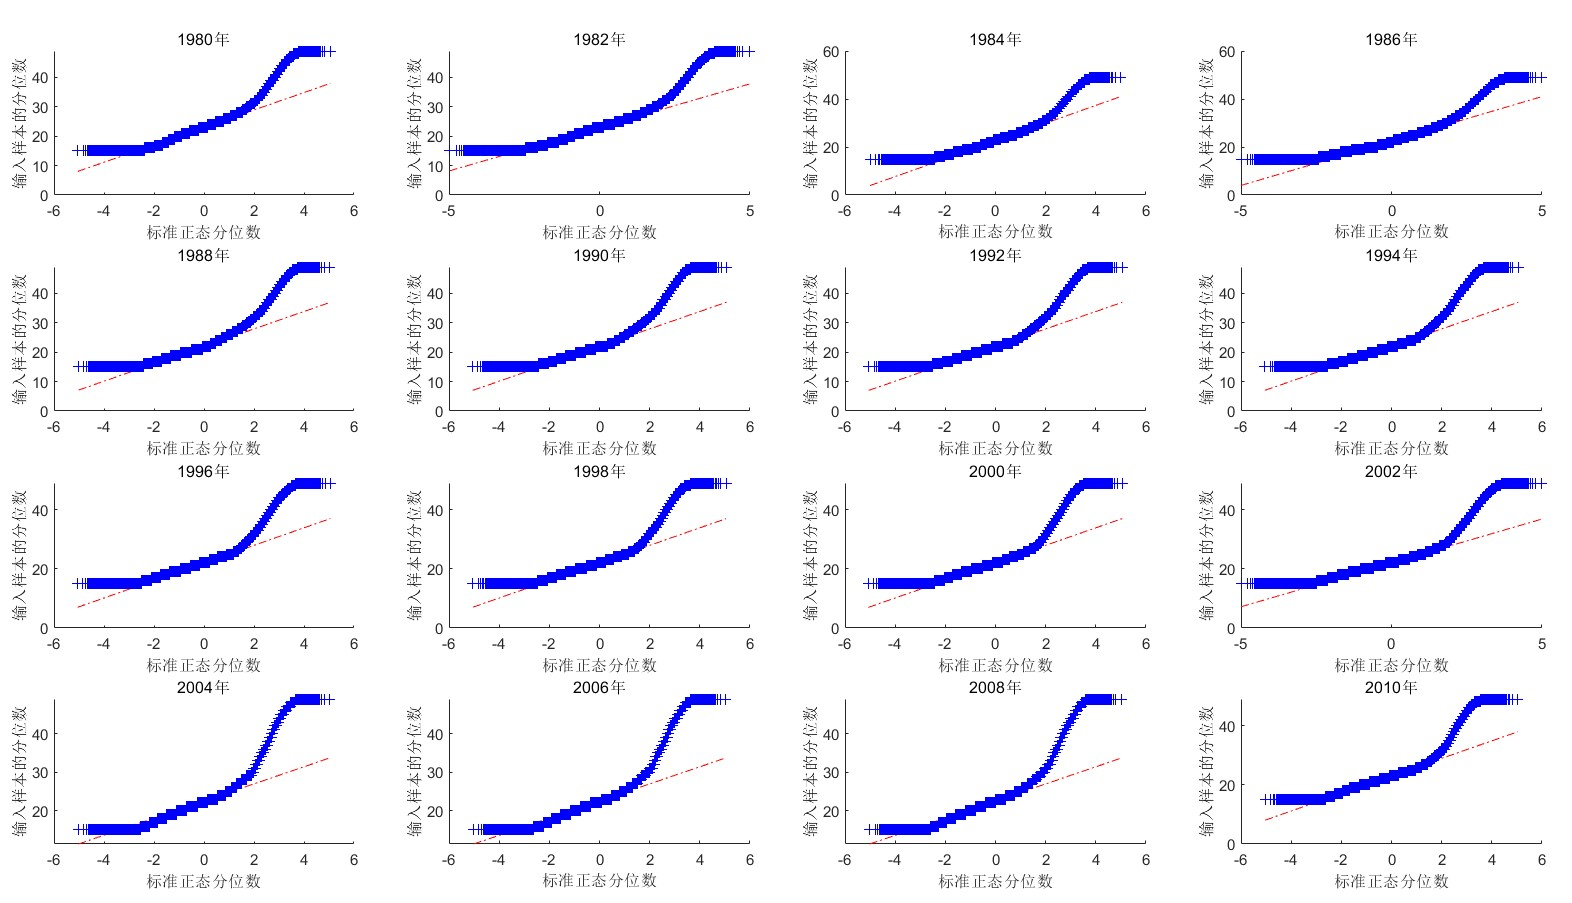
\includegraphics[width=1\textwidth]{004.JPG}
\caption{每个年份的QQ图}
\end{figure}
 
随后,我们计算出他的峰度与偏度,如下图

\begin{figure}[h!]
\centering
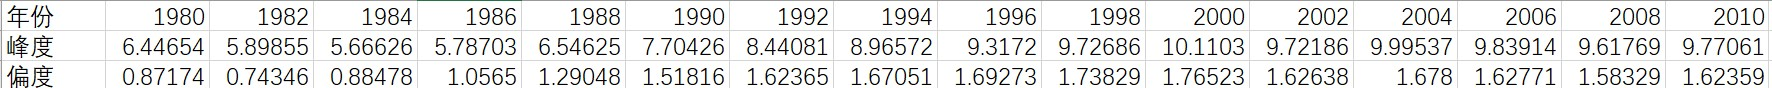
\includegraphics[width=1\textwidth]{005.JPG}
\caption{峰度与偏度}
\end{figure}

正态分布的峰度值为3,偏度为0,而数据中偏度基本在1附近,峰度在6到10不等。

\section{结果分析}
由QQ图可以看出,两边的数据分布相比正态分布较多,中间部分与正态分布较为相近。但是检验不通过,且QQ图中分布并非相对集中于直线上,判断为不服从正态分布。由峰度与偏度的计算结果可见,重尾在右侧时,该分布偏向右侧,因为法律的限制以及社会的传统,初婚年龄集中分布在25岁左右,大家结婚年龄相对集中,一是中国人口基数大,二是社会的传统。


\begin{thebibliography}{99}  

\bibitem{ref1}\href{http://www.stats.gov.cn/tjsj/pcsj/rkpc/6rp/indexch.htm}{中国2010年人口普查资料}
\addcontentsline{toc}{section}{参考文献}
\end{thebibliography}

\textbf{MATLAB代码}

\begin{lstlisting}
%%绘制隔2年与隔4年的数据图
[num,txt,raw]=xlsread('D:\Desktop\B0504a.xls');%读取数据表格
raw
x=[];
for i=1:16
    x=[x,cell2mat(raw(9:43,5+(i-1)*3))];
end
y0=15:49;
for j=1:16
    plot(y0,x(:,j));
    k=1980+(j-1)*2;
    str{j}=[num2str(k),'年'];
    hold on
end
legend(str);
xlabel('初婚年龄');
ylabel('结婚人数');
title('1980-2010隔2年的统计');
hold off

for j=1:8
    plot(y0,x(:,j*2-1),'LineWidth',2);
    k=1980+(j*2-2)*2;
    str{j}=[num2str(k),'年'];
    hold on
end
legend(str);
xlabel('初婚年龄');
ylabel('结婚人数');
title('1980-2010隔4年的统计');
hold off


%%绘制单独图像
[num,txt,raw]=xlsread('D:\Desktop\B0504a.xls');%读取数据表格
raw
x=[];
for i=1:16
    x=[x,cell2mat(raw(9:43,5+(i-1)*3))];
end
y0=15:49;
for j=1:16
    subplot(4,4,j)
    plot(y0,x(:,j));
    k=1980+(j-1)*2;
    title([num2str(k),'年']);
end

%%绘制qq图
[num,txt,raw]=xlsread('D:\Desktop\B0504a.xls');%读取数据表格
raw
x=[];
for i=1:16
    x=[x,cell2mat(raw(9:43,5+(i-1)*3))];
end
y0=15:49;
for j=1:16
    y=[];
    for m=1:35
        y=[y,ones(1,x(m,j))*y0(m)];
    end
    subplot(4,4,j)
    qqplot(y);
    k=1980+(j-1)*2;
    title([num2str(k),'年']);
end

%%绘制直方图
[num,txt,raw]=xlsread('D:\Desktop\B0504a.xls');%读取数据表格
raw
x=[];
for i=1:16
    x=[x,cell2mat(raw(9:43,5+(i-1)*3))];
end
y0=15:49;
for j=1:16
    y=[];
    for m=1:35
        y=[y,ones(1,x(m,j))*y0(m)];
    end
    subplot(4,4,j)
    histogram(y);
    k=1980+(j-1)*2;
    title([num2str(k),'年']);
end

%%峰度与偏度计算
[num,txt,raw]=xlsread('D:\Desktop\B0504a.xls');%读取数据表格
raw
x=[];
for i=1:16
    x=[x,cell2mat(raw(9:43,5+(i-1)*3))];
end
y0=15:49;
for j=1:16
    y=[];
    for m=1:35
        y=[y,ones(1,x(m,j))*y0(m)];
    end
    y_kurtois=kurtosis(y)%峰度
    y_sknew=skewness(y)%偏度
end

%%正态检验jb检验
[num,txt,raw]=xlsread('D:\Desktop\B0504a.xls');%读取数据表格
raw
x=[];
for i=1:16
    x=[x,cell2mat(raw(9:43,5+(i-1)*3))];
end
y0=15:49;
for j=1:16
    y=[];
    for m=1:35
        y=[y,ones(1,x(m,j))*y0(m)];
    end
    [h,p]=jbtest(y,0.5);
end
\end{lstlisting}
\end{document}



